  \documentclass[12pt]{article}
 
\usepackage[margin=1in]{geometry}
\usepackage{amsmath,amsthm,amssymb}
\usepackage[spanish]{babel}
\decimalpoint
\usepackage[utf8]{inputenc}
\usepackage{enumitem, kantlipsum}
\usepackage{graphicx}
\setlength{\parindent}{0cm} 

\begin{document}
 
\begin{center}
\Large \textbf{C.Física Moderna: Taller 4}\\
\normalsize \textbf{Mecánica relativista y ''Relatividad general"}
\end{center}
 
  

\section{Fuerza}


 Una carga $q$ en $x = 0$ se acelera desde el reposo debido a un campo eléctrico constante
$\vec{E} = E \;\hat{x}$,
con $E > 0$.

\begin{enumerate}
	\item Muestre que la aceleración de la carga está dada por:
	\begin{equation}
	a_x = \frac{q E}{m_0} (1-u_x^2/c^2)^{3/2}
	\end{equation}
	\item  Muestre que la velocidad de la carga en cualquier tiempo $t$ está dado por:
	\begin{equation}
	u_x = \frac{qEt/m_0}{\sqrt{1+(qEt/m_0 c)^2}}
	\end{equation}
	(Ayuda: Integre la fuerza directamente)
	\item Muestre que la distancia que se ha movido la carga a un tiempo $t$ está dada por:
	\begin{equation}
	x(t) = \frac{m_0 c^2}{qE} \left(\sqrt{1+(qEt/m_0c)^2}-1\right)
	\end{equation}
	\item  Muestre que cuando $t$ es grande, $u_x$ tiende a $c$ \& $x = ct$.
	\item  Muestre que si $qEt/m_0 \ll c$ se obtienen los resultados clásicos para $a_x , u_x$ y $x$.
\end{enumerate}



\noindent\rule{16.5cm}{0.4pt}


\begin{center}
	\textbf{Solución}
\end{center}


1. Para calcular se procede a derivar la fuerza relativista:

\begin{equation}
\frac{d( m_0 v \gamma)}{dt} = m_0 \left(v\frac{d\gamma}{dt}+ a \gamma\right)
\end{equation}


\begin{align}
\frac{d\gamma}{dt} &= \frac{du}{dt} \frac{d\gamma}{du}\\
 &= a \frac{u/c^2}{(1-(u/c)^2)^{3/2}} \\
 &=a \gamma^3
\end{align}


\begin{align}
v\frac{d\gamma}{dt}+ a \gamma &= a \gamma\left(  \frac{(u/c)^2}{1-(u/c)^2}+1\right)\\
&= a\gamma^{3}
\end{align}

Por lo que:

\begin{equation}
F = m_0 a \gamma^3
\end{equation}

Y la fuerza eléctrica es $F = q E$. Luego

\begin{align}
a_x = \frac{q E}{m_0 \gamma^3} \\
&=\frac{q E}{m_0} (1-u_x^2/c^2)^{3/2}
\end{align}


2. Utilizando $F = dp/dt = q E$, se integra directamente:

\begin{equation}
m_0 u \gamma = qEt  
\end{equation}

Elevando al cuadrado:


\begin{equation}
 u^2  = \left(\frac{qEt}{m_0}\right)^2 (1-u^2/c^2)
\end{equation}

Agrupando $u^2$:

\begin{equation}
u^2\left(  1 + \left(\frac{qEt}{m_0 c}\right)^2\right)  = \left(\frac{qEt}{m_0}\right)^2 
\end{equation}

Finalmente se obtiene:

\begin{equation}
u^2  = \frac{\left(\frac{qEt}{m_0}\right)^2}{  1 + \left(\frac{qEt}{m_0 c}\right)^2} 
\end{equation}

Sacando la raíz cuadrada se obtiene el resultado.


\section{Relatividad general}

\begin{enumerate}
	\item  Desde el punto de vista de un sistema de referencia con aceleración (a); un rayo de luz se desvía como lo
	muestra la siguiente figura:	
	\begin{center}
			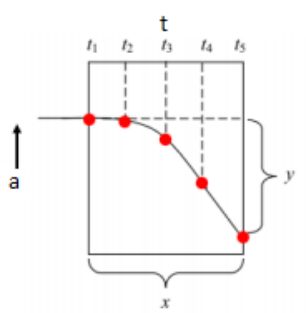
\includegraphics[scale=0.6, angle=0]{1}
	\end{center}
	Calcular la distancia (y) que “cae” un fotón de luz en este sistema de referencia en función de la distancia $x$
	“horizontal” que recorre; sabiendo que el tiempo de aceleración es $t$; use las expresiones clásicas de la
	mecánica.
	\item Obtener la expresión general del valor de la aceleración de la gravedad en la superficie de un cuerpo masivo
	uniforme de masa (m), usando la ley de gravitación universal.
	\item Usando el principio de equivalencia de la relatividad general, además de asumir que el rayo de luz incide
	sobre la superficie del cuerpo, y que la acción de la gravedad afecta al rayo durante una distancia del orden
	del diámetro del cuerpo masivo (mirar figura); demostrar que la desviación de un rayo de luz debida a este es
	($G$: constante de gravitación universal):
		\begin{center}
		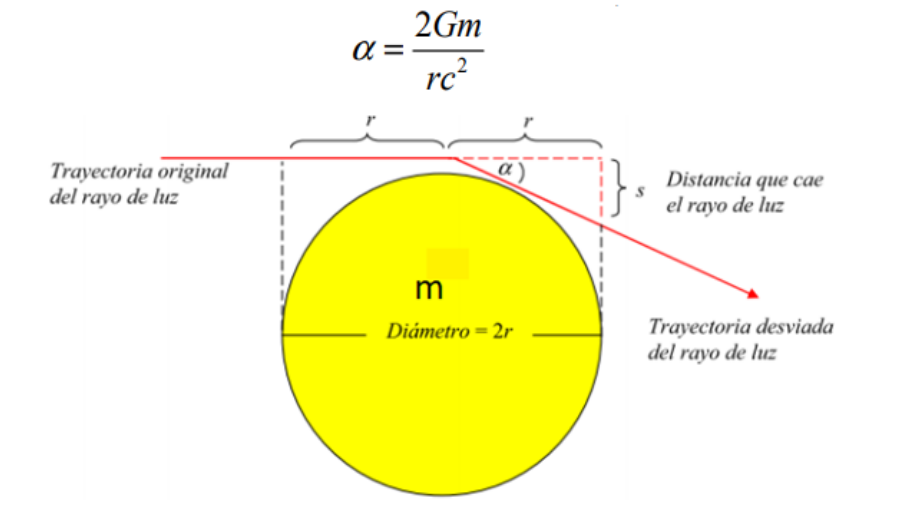
\includegraphics[scale=0.6, angle=0]{2}
	\end{center}
	\item Calcular la desviación de un rayo de luz que incide sobre la superficie del sol en segundos de arco. Usando
	el formalismo de la relatividad general se demuestra que la desviación real es el doble que la anterior
	deducida, explique este este hecho.
\end{enumerate}





\noindent\rule{16.5cm}{0.4pt}




\begin{center}
\textbf{Fórmulas útiles}
\end{center}




\textbf{Fuerza relativista}\\



\begin{align*}
F_x = \frac{d p_x}{dt}
\end{align*}


Donde

\begin{align*}
p_x = m u \gamma
\end{align*}

Integral útil: $$  \int dx  \frac{x}{\sqrt{1-\zeta x^2}} = -\frac{\sqrt{1-\zeta x^2}}{\zeta}$$


\end{document}